\subsection{Human data results}\label{app:human}

\begin{table}[H]
  \centering
  \sffamily
  \small
  \tabcolsep=0.11cm
  \begin{tabular}{
    @{}
    l
    S[table-format=2]
    S[table-format=3]
    S[table-format=3]
    S[table-format=3]
    S[table-format=1.1]
    S[table-format=1.1]
    S[table-format=2.1]
    S[table-format=1.2]
    S[table-format=1.1]
    S[table-format=2]
    @{}
    }
    \toprule
    &
    & \multicolumn{3}{c}{\textbf{Length} [\kbp]}
    & \multicolumn{3}{c}{\textbf{Divergence} [$\%$]}
    & \multicolumn{3}{c}{\textbf{Max gap} [\kbp]}
    \\
    \cmidrule(lr){3-5} \cmidrule(lr){6-8} \cmidrule(lr){9-11}
    \textbf{Dataset}
    & {\!\!\textbf{Cnt}} &
    {\small min} & {\small \!mean} & {\small max} &
    {\small min} & {\small \!mean\!} & {\small max} &
    {\small min} & {\small \!mean\!} & {\small max} \\
    \midrule
    ONT & 50
     & 500 & 594 & 849 & 2.7 & 6.3 & 18.0 & 0.02 & 0.1 & 1 \\
    ONT+gen.var.\!\! & 48
     & 502 & 632 & 1053 & 4.4 & 7.4 & 19.8 & 0.05 & $\mathbf{1.9}$ & $\mathbf{42}$ \\
    \bottomrule
  \end{tabular}
  \caption[Human datasets statistics.]{\textbf{Human datasets statistics.} ONT reads only include short
    gaps, while genetic variation also includes long gaps. \textbf{Cnt}: number of
    sequence pairs. \textbf{\mbox{Max gap}}: longest gap in the reconstructed
    alignment.}
  \label{tab:hg}
\end{table}

\begin{figure*}[H]
  \centering
  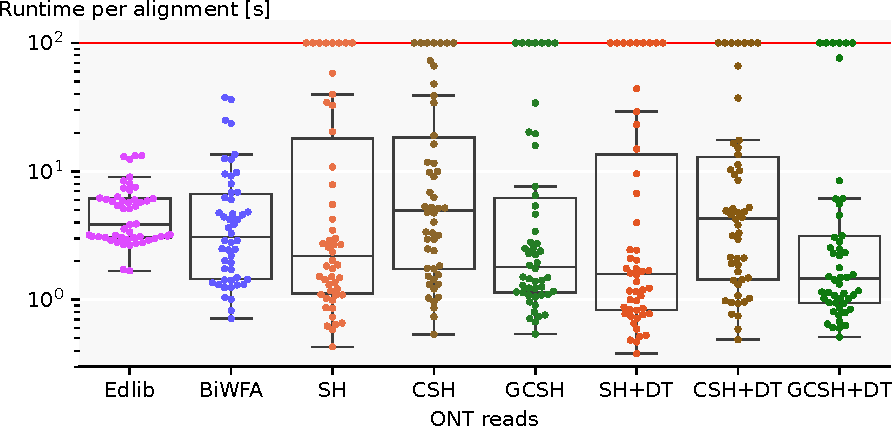
\includegraphics[scale=0.55]{plots/real_full_without_bio_var.pdf}\\
  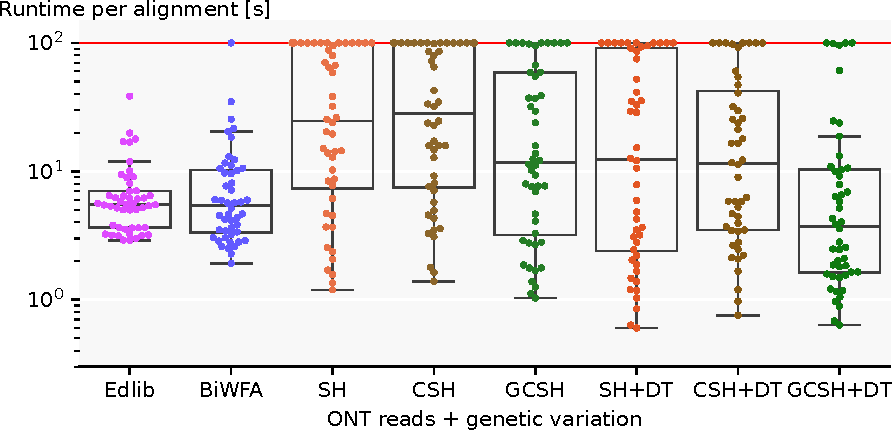
\includegraphics[scale=0.55]{plots/real_full_with_bio_var.pdf}%
  \caption[Runtime on long reads of human data]{\textbf{Runtime on long reads of
    human data} (logarithmic, $\geq 500\kbp$). Each dot corresponds to an
    alignment of a sequence pair. The ONT reads are without (top) and with
    (bottom) genetic variation. Runtime is capped at $\qty{100}{s}$.}
  \label{fig:human-full}
\end{figure*}

Statistics on our human data are presented in~\cref{tab:hg}. We compare all our
heuristics in~\cref{fig:human-full}.

For ONT reads without genetic variation, \SH is faster than other methods in
median, but slower for sequences with high divergence and larger gaps.
\CSH is slightly slower than \SH due to additional bookkeeping without
significant benefit for the heuristic. Penalizing indels with \GCH improves
performance several times.

When genetic variation is included, \SH and \CSH do not sufficiently penalize
long gaps, and \A with \GCH estimates the remaining edit distance significantly
better. The diagonal transition optimization considerably speeds up the
alignment of long indels where the search regresses to quadratic.
